\documentclass{article}
\usepackage{main}

\title{Acticité : Représentation graphique de fonctions}
\author{Seconde 9}
\date{3 Mars 2025}

\begin{document}
\maketitle

\section{Repère orthonormé}
\begin{center}
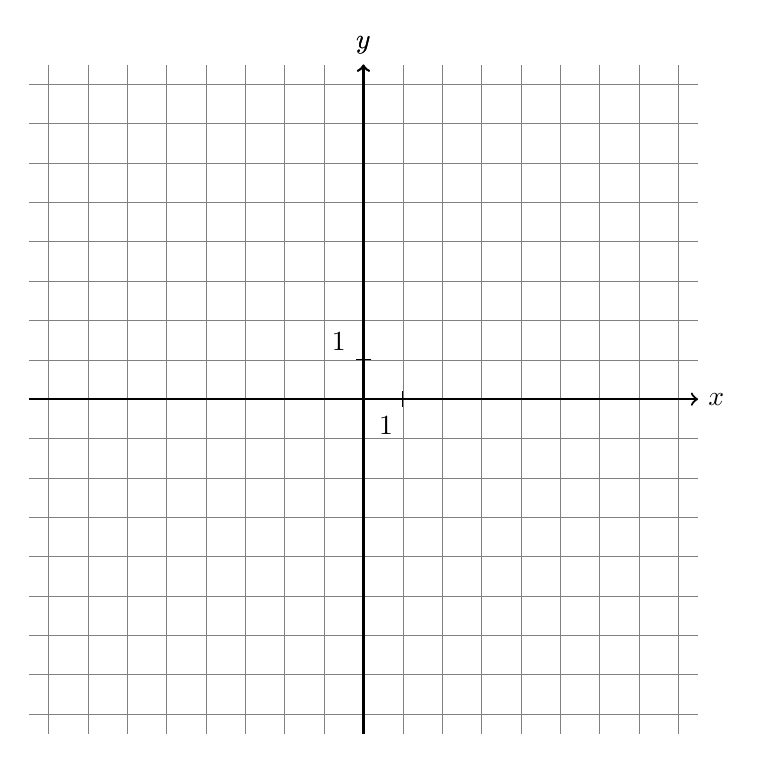
\begin{tikzpicture}
\draw[help lines] (-4.25,-4.25) grid[step=0.5] (4.25,4.25);
\draw[thick,->] (-4.25,0) -- (4.25,0) node[right] {$x$};
\draw[thick,->] (0,-4.25) -- (0,4.25) node[above] {$y$};
\draw[thick,->] (0,-4.25) -- (0,4.25) node[above] {$y$};
\draw (0.5,0.1) -- (0.5,-0.1) node[below left] {$1$};
\draw (0.1,0.5) -- (-0.1,0.5) node[above left] {$1$};
\end{tikzpicture}
\end{center}

\begin{enumquestions}
\item Choisissez deux nombres $x$ et $y$. Placer un point $A$ sur le repère capable de correspondre aux deux nombres.

$x=$ \answersline; $y=$ \answersline
\item\label{Choix} Choisissez un nombre $b$ et une fonction $f$ de votre choix.

$b=$ \answersline; $f : x \mapsto$ \answersline

Donner la valeur de $f(b)$. $f(b)=$ \answersline

Placer le point $B$ de coordonnées $(b;f(b))$ (abscisse = $b$; ordonnée = $f(b)$).
\item Recommencer la question \ref{Choix} pour placer trois autres points $C$; $D$; $E$.
\item Relier les points à main levée pour former une courbe. Si $M$ est un point de coordonnées $(x;y)$ appartenant à cette courbe, quelle est la relation entre $x$ et $y$ (soit sous la forme d'une équation, soit sous la forme d'une phrase en français)?

\answersline

\begin{tcolorbox}
La courbe que vous avez dessinée est appelée \textbf{courbe représentative de la fonction $f$}
\end{tcolorbox}

\item (Pour aller plus loin) Tracer sur le repère suivant une courbe qui n'est \textsc{PAS} la courbe représentative d'une fonction.
\begin{center}
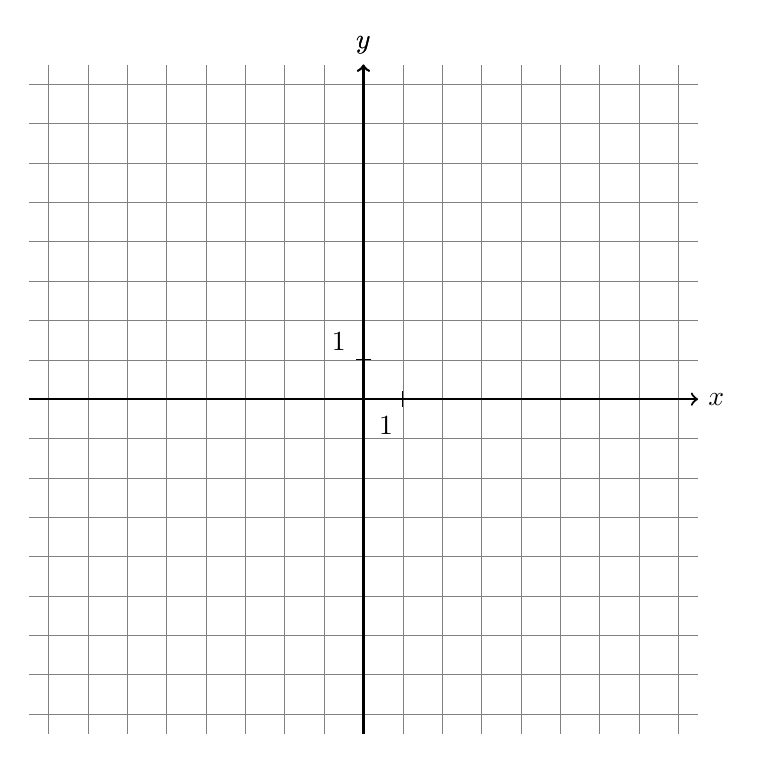
\begin{tikzpicture}
\draw[help lines] (-4.25,-4.25) grid[step=0.5] (4.25,4.25);
\draw[thick,->] (-4.25,0) -- (4.25,0) node[right] {$x$};
\draw[thick,->] (0,-4.25) -- (0,4.25) node[above] {$y$};
\draw[thick,->] (0,-4.25) -- (0,4.25) node[above] {$y$};
\draw (0.5,0.1) -- (0.5,-0.1) node[below left] {$1$};
\draw (0.1,0.5) -- (-0.1,0.5) node[above left] {$1$};
\end{tikzpicture}
\end{center}

\end{enumquestions}

\section{Découverte de la courbe représentative d'une fonction, et son équation}

\includegraphics[width=\textwidth]{Activite.png}
\end{document}